\chapter{\ifproject%
\ifcpe โครงสร้างและขั้นตอนการทำงาน\else Project Structure and Methodology\fi
\else%
\ifcpe โครงสร้างของโครงงาน\else Project Structure\fi
\fi
}

% ในบทนี้จะกล่าวถึงหลักการ และการออกแบบระบบ

\makeatletter

% \renewcommand\section{\@startsection {section}{1}{\z@}%
%                                    {13.5ex \@plus -1ex \@minus -.2ex}%
%                                    {2.3ex \@plus.2ex}%
%                                    {\normalfont\large\bfseries}}

\makeatother
%\vspace{2ex}
% \titleformat{\section}{\normalfont\bfseries}{\thesection}{1em}{}
% \titlespacing*{\section}{0pt}{10ex}{0pt}

\section{User interface (UI)}
User interface (UI) คือการออกแบบที่เน้นไปที่เรื่องหน้าตา ความสวยงาม และทุกอย่างที่จะเป็นการโต้ตอบกับผู้ใช้งาน โดยจะแสดงการเชื่อมโยงของแต่ละหน้าผ่าน user flow ดังรูปที่~\ref{userflow} UI ที่ดีจะช่วยดึงดูดผู้ใช้งานให้เกิดความสนใจและช่วยให้ผู้ใช้งานเข้าถึงข้อมูลได้ง่าย
โดยการออกแบบ UI ของเกมนี้พวกเราจะออกแบบเกมแนวตะลุยไปยังแผนที่ต่างๆ ที่มีสภาพแวดล้อมแตกต่างกัน โดยจะใช้ assets ที่มีอยู่ใน Unity มาปรับแต่งจัดวางเพื่อความสวยงามและความน่าสนใจ โดยจะมีส่วนต่างๆ ดังนี้
\begin{itemize}
\item หน้าจอแสดง main menu (รูปที่ \ref{mainmenu})
\item หน้าจอแสดงหน้าเลือกแผนที่ (รูปที่ \ref{map})
\item หน้าจอแสดงหน้าเลือกด่าน (รูปที่ \ref{stage})
\item หน้าจอแสดงหน้า gameplay (รูปที่ \ref{game})
\item หน้าต่างที่แสดงว่าเราชนะ (รูปที่ \ref{win})
\item หน้าต่างที่แสดงว่าเราแพ้ (รูปที่ \ref{lose})
\end{itemize}

\begin{figure}[h!]
    \begin{center}
    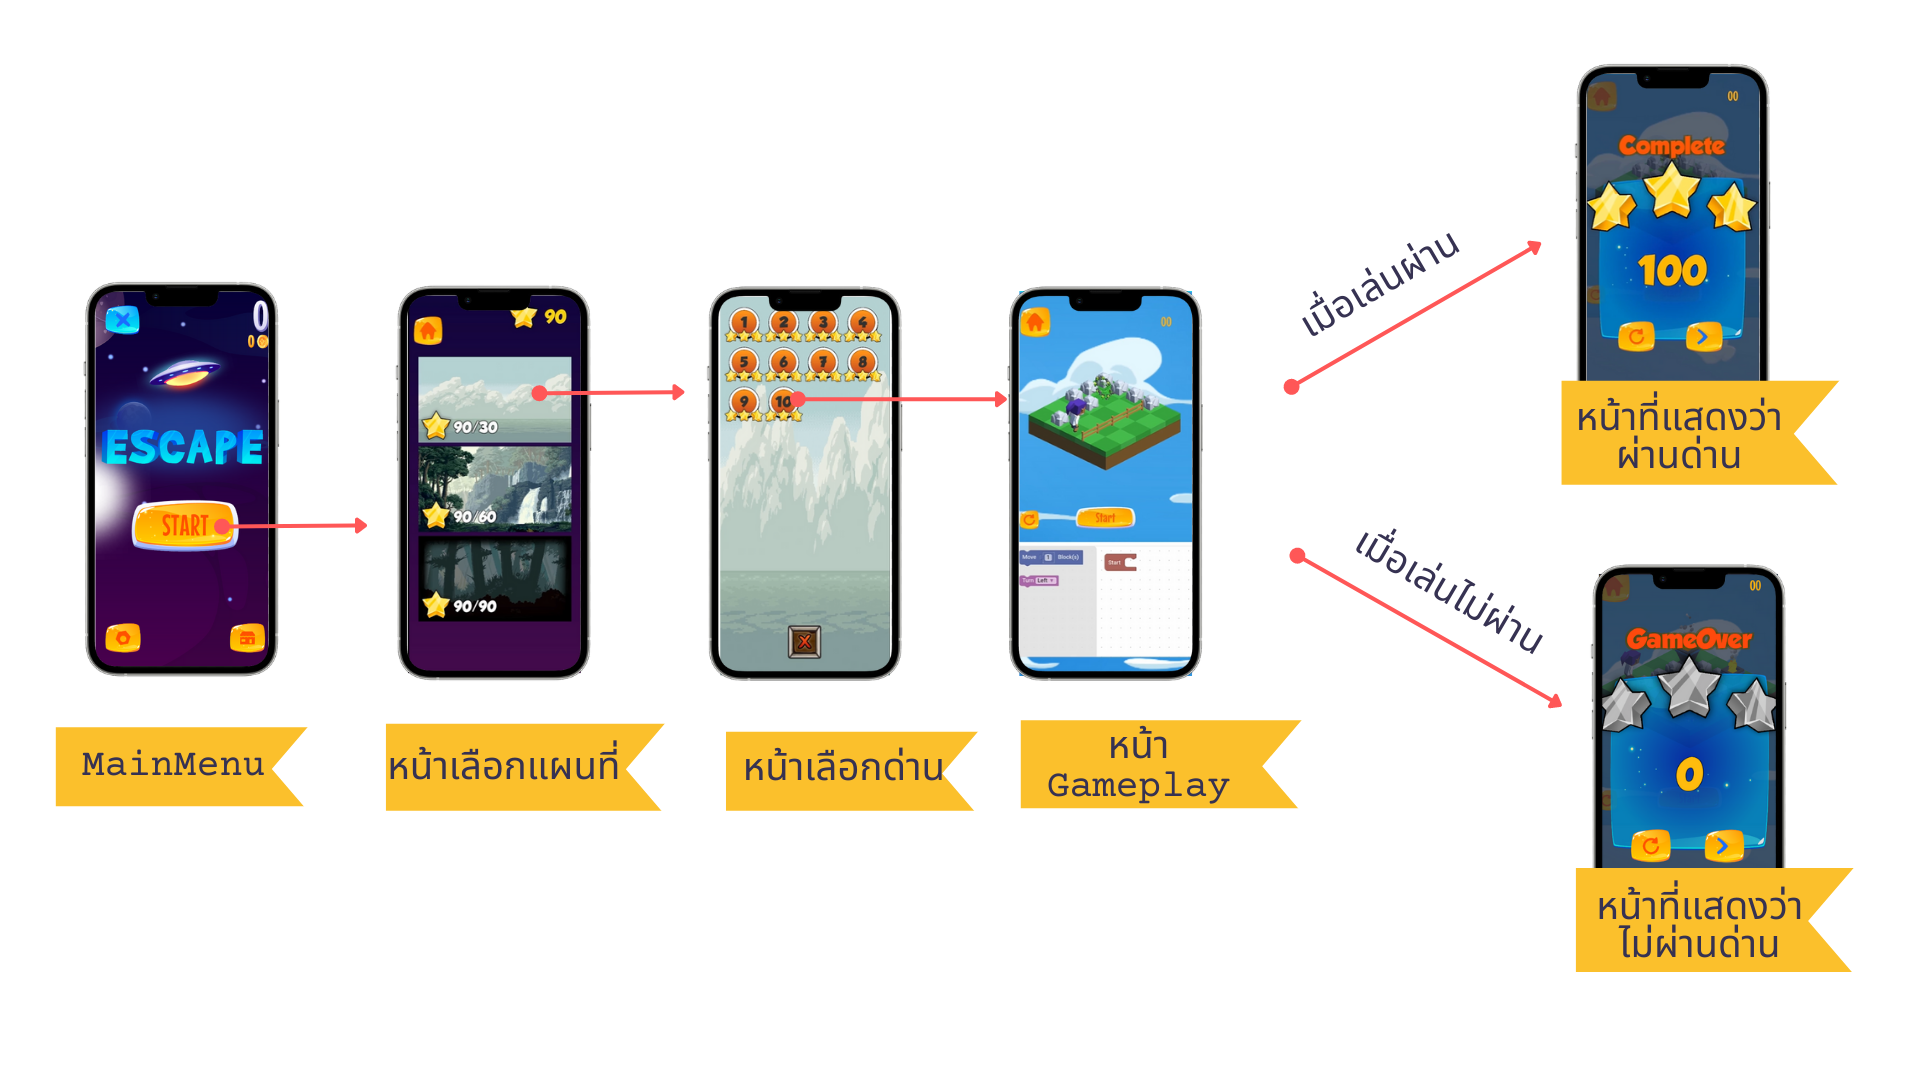
\includegraphics [width=\textwidth] {pic/UXflowchart.png}
    \end{center}
    \caption{User flow}
    \label{userflow}
    \end{figure}

\GBreply{ควรจะเอาขึ้นก่อนไหม? อธิบายด้วย ไม่ใช่ว่าแปะๆๆ อาจจะทำ User Flow ไหม?}
\begin{figure}[h!]
\begin{center}
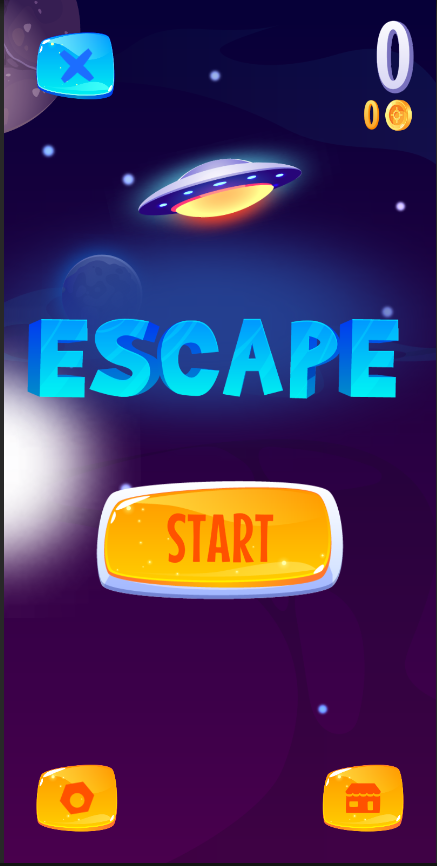
\includegraphics[width=1.75in]{pic/home_start.PNG}
\end{center}
\caption[Mainmenu ของเกม]{หน้า main menu ของเกม}
\label{mainmenu}
\end{figure}


\begin{figure}[h!]
\begin{center}
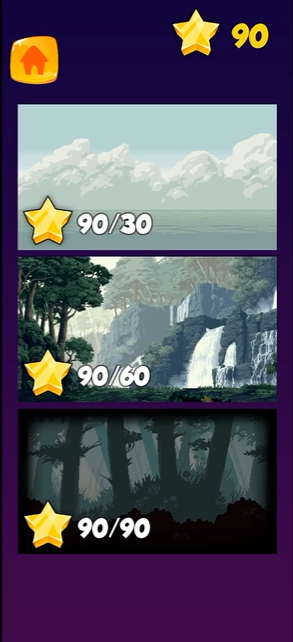
\includegraphics[width=1.75in]{pic/MapSelection.png}
\end{center}
\caption[หน้าเลือกแผนที่]{หน้าเลือกแผนที่}
\label{map}
\end{figure}

\begin{figure}[h!]
\begin{center}
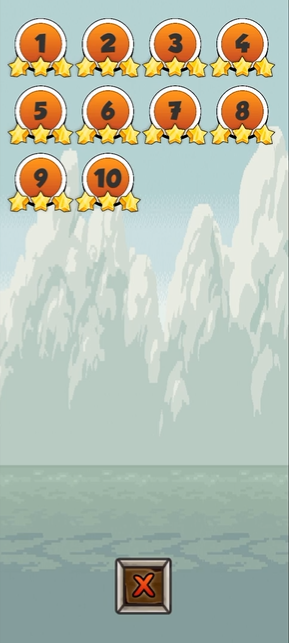
\includegraphics[width=1.75in]{pic/LevelSelection1.png}
\end{center}
\caption[หน้าเลือกด่าน]{หน้าเลือกด่าน}
\label{stage}
\end{figure}


\begin{figure}[h!]
\begin{center}
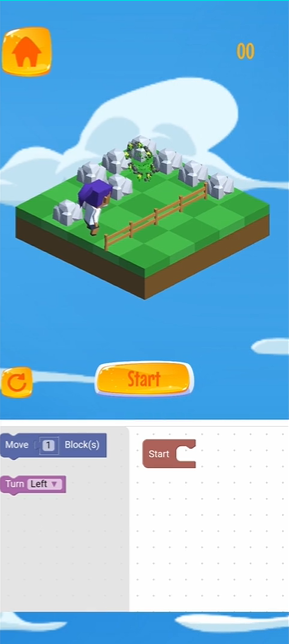
\includegraphics[width=1.75in]{pic/NewGamePlay.png}
\end{center}
\caption[หน้า Gameplay]{หน้า gameplay}
\label{game}
\end{figure}

\begin{figure}[h!]
\begin{center}
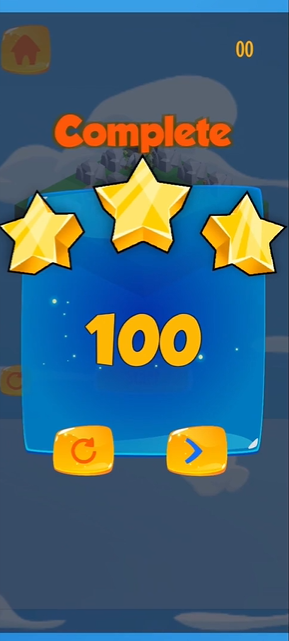
\includegraphics[width=1.75in]{pic/Complete.png}
\end{center}
\caption[หน้าต่างที่แสดงว่าชนะ]{หน้าต่างที่แสดงว่าชนะ}
\label{win}
\end{figure}

\begin{figure}[h!]
\begin{center}
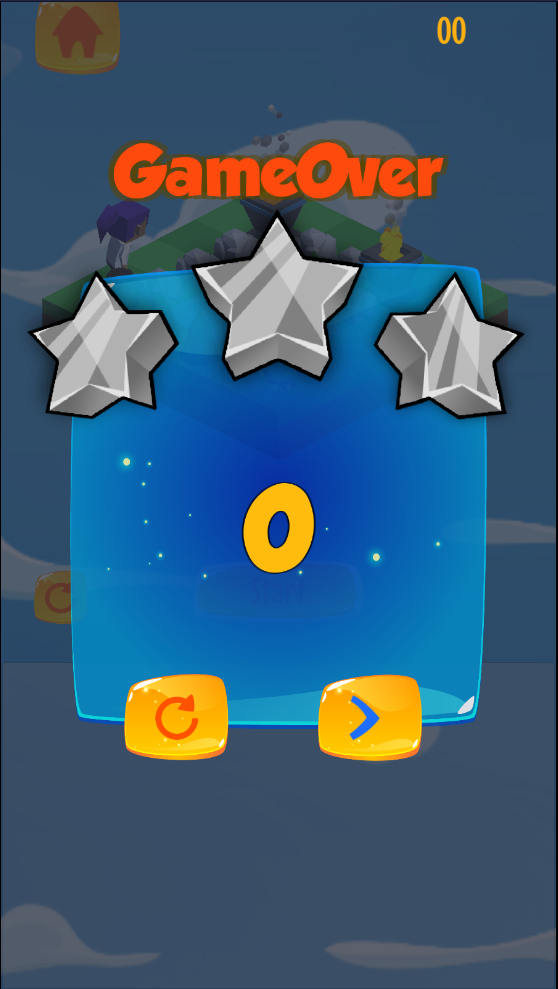
\includegraphics[width=1.75in]{pic/GameOver1.png}
\end{center}
\caption{หน้าต่าง game over}
\label{lose}
\end{figure}

\clearpage

\section{WebView}
เป็นตัวหน้าเว็บสำหรับนำ Google Blockly ไปใส่ใน panel ของ Unity เพราะเดิมที Unity ไม่สามารถสร้าง objects ที่มีหน้าตาและ functions เหมือนกับ Google Blockly ได้ ทางผู้พัฒนาจึงสร้างหน้าเว็บเข้ามาเพื่อนำไปใส่ใน 
panel ของ Unity ที่ใช้ในการแสดงผล block code

\begin{figure}[h!]
\begin{center}
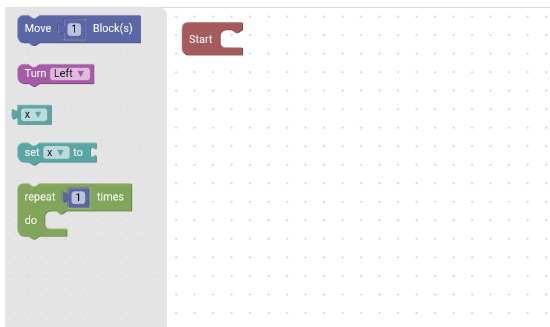
\includegraphics{pic/CodePanel.png}
\end{center}
\caption[Google Blockly]{Google Blockly}
\label{block}
\end{figure}


\section{Text reader}
ด่านต่างๆ ของเกมนี้จะถูกระบุเป็น input ด้วยไฟล์ text กล่าวคือ เมื่อ user ทำการ input ไฟล์มา ตัวระบบเกมจะทำการจัดการสร้างด่านให้เอง
ทำให้การที่จะสร้างด่านหนึ่งด่านไม่ต้องเสียเวลาลากวางตัว prefabs บน Unity รูปที่~\ref{txt} แสดงตัวอย่างไฟล์ text โดยคร่าวๆ\CIreply{อธิบาย file spec โดยคร่าวๆ ด้วย}

\begin{figure}[h!]
    \begin{center}
    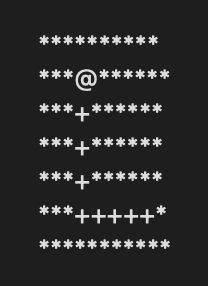
\includegraphics{pic/text.png}
    \end{center}
    \caption[Text]{Text}
    \label{txt}
    \end{figure}
